\section{Results and Discussion}
\begin{table*}[t]
\centering
\caption{Attack detection on the chronological test set (\%, mean$\pm$std over five seeds; best in bold). The test sets contain 347/453/100 (14-bus) and 370/451/79 (118-bus) normal/stealthy/naive snapshots.}
\label{tab:det}
\footnotesize
\setlength{\tabcolsep}{3.2pt}
\begin{tabular}{l cccc cccc}
\toprule
& \multicolumn{4}{c}{IEEE 14-bus} & \multicolumn{4}{c}{IEEE 118-bus}\\
\cmidrule(lr){2-5}\cmidrule(lr){6-9}
Method & Acc. & F1 & FPR $\downarrow$ & AUC & Acc. & F1 & FPR $\downarrow$ & AUC\\
\midrule
BDD (chi-square) & 49.56 & 31.00 & \textbf{0.86} & 58.54 & 49.67 & 26.10 & 0.81 & 57.79 \\
DT-Threshold & 95.67 & 96.39 & 1.73 & 98.34 & 96.00 & 96.50 & \textbf{0.54} & 98.74 \\
SVM-RBF (raw) & 94.78 & 95.62 & 2.02 & 97.71 & 85.78 & 87.33 & 10.54 & 92.58 \\
RandomForest (raw) & 93.24$\pm$0.12 & 94.42$\pm$0.11 & 6.34$\pm$0.29 & 97.38$\pm$0.04 & 81.27$\pm$0.80 & 83.61$\pm$0.61 & 18.49$\pm$1.85 & 89.51$\pm$0.37 \\
MLP (raw) & 93.89$\pm$0.46 & 94.94$\pm$0.36 & 5.19$\pm$1.48 & 97.65$\pm$0.14 & 78.62$\pm$1.34 & 81.19$\pm$0.89 & 20.92$\pm$5.16 & 87.27$\pm$1.10 \\
GCN (raw) & 93.09$\pm$0.14 & 94.13$\pm$0.14 & 2.42$\pm$0.85 & 96.81$\pm$0.15 & 91.84$\pm$0.10 & 92.66$\pm$0.10 & 1.84$\pm$0.59 & 94.86$\pm$0.22 \\
DT-MLP & 95.58$\pm$0.43 & 96.36$\pm$0.34 & 3.75$\pm$1.37 & 98.61$\pm$0.07 & 85.29$\pm$0.90 & 87.05$\pm$0.78 & 12.86$\pm$4.84 & 92.96$\pm$0.37 \\
DT-GCN (prop.) & \textbf{97.27$\pm$0.24} & \textbf{97.75$\pm$0.19} & 1.96$\pm$0.69 & \textbf{99.23$\pm$0.06} & \textbf{97.04$\pm$0.36} & \textbf{97.45$\pm$0.31} & 1.35$\pm$0.43 & \textbf{99.00$\pm$0.05} \\
\bottomrule
\end{tabular}
\end{table*}

\begin{table*}[t]
\centering
\caption{Localization of compromised buses on stealthy test attacks (\%, mean$\pm$std over five seeds).}
\label{tab:loc}
\footnotesize
\begin{tabular}{l ccc ccc}
\toprule
& \multicolumn{3}{c}{IEEE 14-bus} & \multicolumn{3}{c}{IEEE 118-bus}\\
\cmidrule(lr){2-4}\cmidrule(lr){5-7}
Method & Recall & F1 & Exact match & Recall & F1 & Exact match\\
\midrule
DT-Threshold & 82.34 & 52.63 & 2.65 & 84.02 & 49.13 & 2.88 \\
MLP (raw) & 90.99$\pm$0.54 & 79.21$\pm$2.02 & 34.97$\pm$7.32 & 43.20$\pm$3.67 & 32.58$\pm$1.30 & 0.62$\pm$0.62 \\
GCN (raw) & 87.61$\pm$0.41 & 60.22$\pm$0.97 & 13.95$\pm$1.89 & 84.18$\pm$0.50 & 39.71$\pm$1.03 & 2.00$\pm$0.41 \\
DT-MLP & 94.13$\pm$0.33 & \textbf{89.26$\pm$1.80} & 66.18$\pm$6.38 & 74.48$\pm$2.96 & 45.58$\pm$0.98 & 1.86$\pm$0.60 \\
DT-GCN (prop.) & \textbf{95.93$\pm$0.20} & 89.22$\pm$0.92 & \textbf{77.53$\pm$1.78} & \textbf{94.46$\pm$0.66} & \textbf{79.35$\pm$3.55} & \textbf{50.78$\pm$5.92} \\
\bottomrule
\end{tabular}
\end{table*}

\subsection{Detection Performance}
Table~\ref{tab:det} and Fig.~\ref{fig:roc} summarize detection. The $\chi^2$ BDD catches 100.00\% and 96.20\% of naive attacks. It detects only 0.44\% and 0.89\% of stealthy FDIAs, which is no better than its 1\% nominal false-alarm rate. This confirms that the generated attacks are AC-stealthy. On the 14-bus system all learning-based detectors exceed 94\% F1. Because the model is small, raw-telemetry classifiers can still learn the narrow normal range of each bus injection. The proposed DT-GCN reaches the highest F1 (97.75\%) and AUC (99.23\%).

The advantage widens on the 118-bus system. There, 726 measurements and strongly varying PV and load make the raw-data decision surface much harder. SVM, RF and MLP on raw telemetry fall to 81--87\% F1 with FPR above 10\%. The GCN on raw telemetry reaches 92.66\% F1. DT-GCN keeps 97.45\% F1 at 1.35\% FPR, with AUC 99.00\%. Fig.~\ref{fig:roc} shows that DT-GCN holds about 95\% true-positive rate even at $10^{-3}$ FPR, which matters for operators who must keep alarm fatigue low.

The ablations separate the two ingredients. The learning-free DT-Threshold is already strong (F1 96.50\% on 118-bus), so the twin residuals themselves carry most of the detection signal. Removing the graph (DT-MLP) \emph{hurts} on the large system (87.05\% F1). A flattened 708-dimensional input overfits the 4200 training snapshots, while the topology-shared GCN weights scale to large networks.

\begin{figure*}[t]
\centering
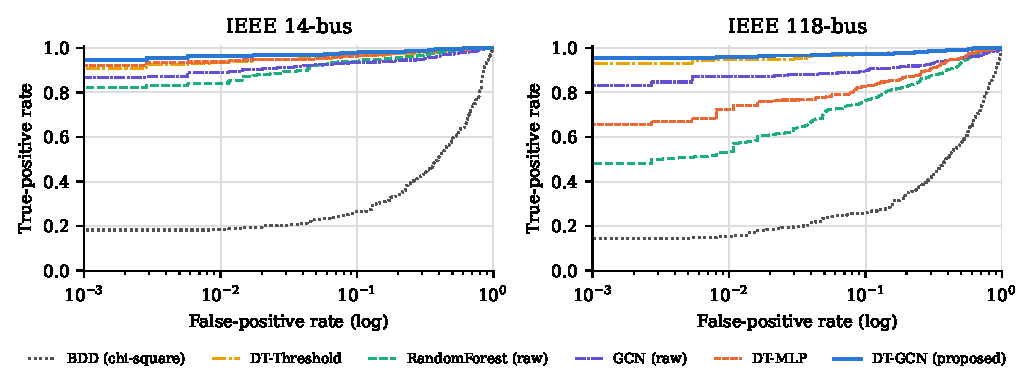
\includegraphics[width=0.92\textwidth]{../figures/roc.pdf}
\caption{ROC curves (log-scaled FPR) on the test set.}
\label{fig:roc}
\end{figure*}

\begin{figure*}[t]
\centering
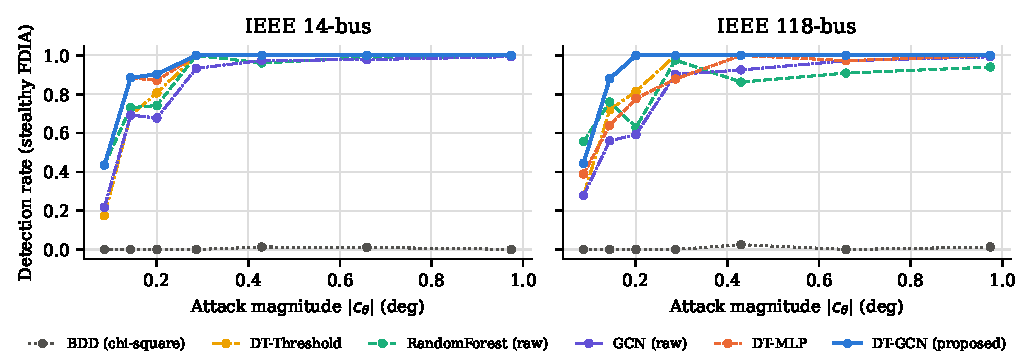
\includegraphics[width=0.92\textwidth]{../figures/recall_mag.pdf}
\caption{Detection rate of stealthy FDIAs versus angle-bias magnitude.}
\label{fig:mag}
\end{figure*}

\subsection{Sensitivity to Attack Strength and Size}
Fig.~\ref{fig:mag} breaks the detection rate down by the injected angle bias. The twin-based detectors find essentially all attacks above about $0.3^\circ$. The raw-telemetry RF still misses 6--14\% of them on the 118-bus system. In the hardest bin ($0.06^\circ$--$0.11^\circ$, comparable to the twin's own angle error) no detector exceeds 56\%, which marks the detectability floor set by twin fidelity and noise. The proposed method gains most between $0.11^\circ$ and $0.23^\circ$ on the 118-bus system. There, DT-GCN detects 88\% and 100\% of attacks in the two bins, while the best competitor detects 76\% and 82\%. On the 14-bus system, DT-GCN and DT-MLP perform similarly in this range (87--90\%). For attacks spanning $k=1,2,3$ buses on the 118-bus system, DT-GCN detects 98.0/96.8/96.5\%, compared with 78.0/90.5/95.1\% for RF on raw telemetry. Single-bus attacks are therefore not harder for the proposed method, whereas raw-data methods lose up to 17 percentage points on them.

\begin{figure}[!t]
\centering
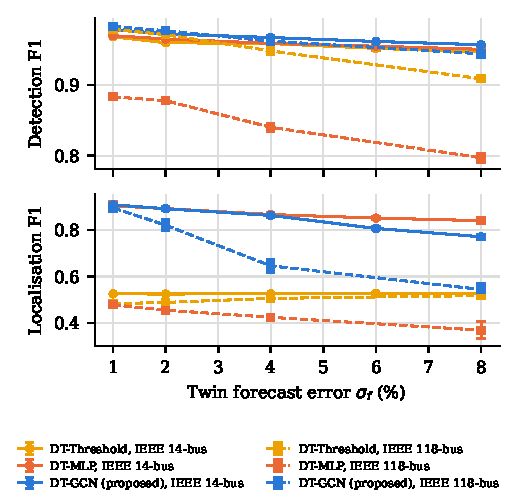
\includegraphics[width=\columnwidth]{../figures/sensitivity.pdf}
\caption{Effect of twin forecast error $\sigma_f$ on detection and localization (solid: 14-bus, 3 seeds; dashed: 118-bus, 2 seeds).}
\label{fig:sens}
\end{figure}

\subsection{Localization}
Table~\ref{tab:loc} reports bus-level localization, where DT-GCN gives the clearest gain. On the 118-bus system it achieves 79.35\% F1 and identifies the \emph{exact} compromised bus set in 50.78\% of attacks. The best alternative reaches 49.13\% F1 and below 3\% exact match. The threshold detector has high recall but poor precision: an attack on bus $i$ also perturbs residuals at its neighbors. Message passing over the topology lets the GCN learn which bus of a disturbed neighborhood is the \emph{source}. On the 14-bus system, DT-GCN and DT-MLP have similar F1 (89.22\% vs 89.26\%), but DT-GCN's exact-match rate is 11 points higher (77.53\%). Fig.~\ref{fig:loc} shows a correctly localized three-bus attack (buses 5, 6 and 13).

\begin{figure}[t]
\centering
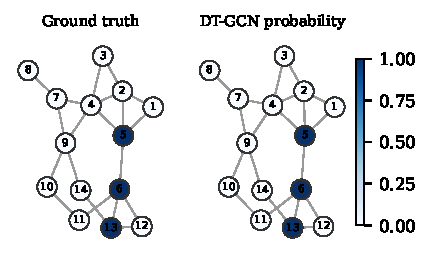
\includegraphics[width=0.85\columnwidth]{../figures/localisation.pdf}
\caption{Localization of a three-bus stealthy FDIA on the IEEE 14-bus system.}
\label{fig:loc}
\end{figure}

\begin{figure}[t]
\centering
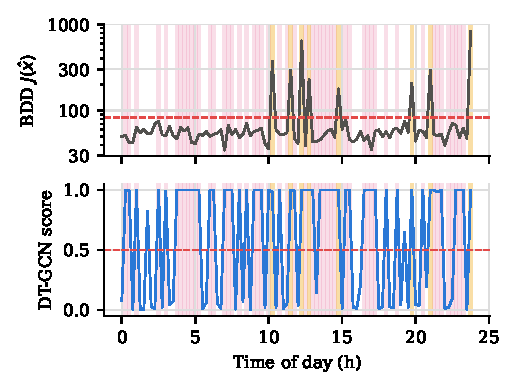
\includegraphics[width=\columnwidth]{../figures/timeline.pdf}
\caption{One test day on the IEEE 14-bus system. Pink: stealthy FDIA intervals; amber: naive attacks; dashed: alarm thresholds. The BDD (top) responds only to naive attacks. DT-GCN (bottom) flags both.}
\label{fig:time}
\end{figure}

\subsection{Sensitivity to Digital-Twin Fidelity}\label{sec:sens}

The method depends on the twin being accurate. Fig.~\ref{fig:sens} retrains the DT-based detectors with the twin's forecast error swept from 1\% to 8\%. For each level the twin is re-simulated with a new forecast-error realization. Detection degrades gracefully. On the 14-bus system DT-GCN keeps 97.9\%, 96.7\% and 95.7\% F1 at $\sigma_f=1$, 4 and 8\%, so even at 8\% it matches the best raw-telemetry detector (SVM, 95.6\%). On the 118-bus system it drops from 98.3\% to 94.4\% F1, compared with 97.9\% to 90.9\% for DT-Threshold and 88.3\% to 79.7\% for DT-MLP. The graph model is therefore the most robust \emph{detector} when the twin is imperfect. Localization is more sensitive. On the 118-bus system, DT-GCN's bus-level F1 falls from 89.5\% ($\sigma_f=1\%$) to 64.6\% (4\%) and 54.4\% (8\%), approaching the twin-threshold level of about 50\%. On the 14-bus system the decline is milder (90.8\% to 77.1\%), and there DT-MLP degrades less (84.0\% at 8\%). Accurate localization in large networks therefore requires a well-calibrated twin, with nodal forecast errors of a few percent. This is a practical design target for DT-enabled control centers.

\subsection{Computational Cost and Deployment}
The twin power flow, WLS estimation and feature extraction take about 30~ms per snapshot on the 118-bus system in our pure-Python implementation. Batched DT-GCN inference takes 0.078~ms per snapshot. The whole chain is therefore far inside a 15-min (or even a 1-s PMU) SE cycle. The model has 25.7k parameters and runs on a commodity CPU. In practice it would run in parallel with the existing BDD, as a second line of defense that needs no change to the SE. The bus-level output can trigger targeted measures, such as re-authenticating the remote terminal units at the flagged buses or temporarily replacing their measurements with twin pseudo-measurements.

\subsection{Limitations}
This study uses simulated data on standard test systems. Load, PV and forecast errors follow parametric models. The attacker is assumed not to compromise the forecast and scheduling channels that feed the twin; an adversary who can also bias the twin inputs is outside this threat model. Topology changes and parameter errors in the twin were not modeled. Detectors were trained with labeled attacks, so robustness to attack strategies unseen in training should be checked with semi-supervised or one-class variants. These are planned extensions toward field validation on utility data.

\section{Conclusion}
This paper presented DT-GCN, a digital-twin-assisted graph learning framework for detecting and localizing stealthy AC false data injection attacks. A forecast-driven physics twin supplies an attack-independent reference state. Its bus-level residuals turn a hard anomaly-detection problem in raw telemetry into a well-conditioned graph problem. On the IEEE 14- and 118-bus systems with realistic load/PV variability, a nonlinear WLS estimator and AC-stealthy attacks invisible to the $\chi^2$ test, DT-GCN achieved 97.75\% and 97.45\% detection F1. On the 118-bus system it localized the exact compromised buses in 50.78\% of attacks, outperforming SVM, random forest, MLP and GCN detectors on raw telemetry and the learning-free twin threshold. Future work will cover twin-input integrity, topology attacks, PMU-rate operation, and hardware-in-the-loop validation.
